% \documentclass{report}
% \usepackage[utf8]{inputenc}
% \usepackage[brazil]{babel}

\documentclass[oneside,a4paper,12pt]{normas-utf-tex}

\usepackage{breakurl}
\usepackage[alf,abnt-emphasize=bf,bibjustif,recuo=0cm, abnt-etal-cite=2]{abntcite}
\usepackage[brazil]{babel}
\usepackage[utf8]{inputenc}
\usepackage{amsmath}
\usepackage{graphicx,subfig}
\usepackage{times}
\usepackage[plain]{fancyref}
\usepackage{float}
\usepackage{pdfpages}
\usepackage{enumitem}
\usepackage{longtable}

%%% Complemento para tabelas
\usepackage{booktabs, multirow}
\setlength{\heavyrulewidth}{0.1em}
\renewcommand{\toprule}{\midrule[\heavyrulewidth]}
\renewcommand{\arraystretch}{1.2}
%%%

\instituicao{Universidade Tecnológica Federal do Paraná}
\departamento{Departamento Acadêmico de Eletrônica}
\departamentodois{Departamento Acadêmico de Informática}
\programa{Curso de Engenharia de Computação}
\unidade{Oficina de Integração 3}

\titulo{\MakeUppercase{Mapeamento de ambientes com o robô Bellator}}
\documento{Análise tecnológica}

\autor{Luis Guilherme Machado Camargo}
\autordois{Pedro Alberto de Borba}
\autortres{Ricardo Farah}
\autorquatro{Stefan Campana Fuchs}
\autorcinco{Telmo Friesen}

\cita{CAMARGO, L.G.M; BORBA, P.A.; FARAH, R.; FUCHS, S.C.; FRIESEN, T}

\comentario{\UTFPRdocumentodata\ apresentada à Unidade Curricular de \UTFPRunidadedata\ do \UTFPRprogramadata\ da \ABNTinstituicaodata\ como requisito parcial para aprovação.}

\local{Curitiba}
\data{\the\year}

\begin{document}

\capa
\folhaderosto
\sumario
\chapter{Declaração do Escopo em Alto Nível}

O projeto apresentado neste documento trata-se do “Mapeamento de Ambientes com o robô Bellator” e é uma extensão do projeto “Bellator”. Ele teve sua última alteração em 2012 quando foi utilizado por Alexandre Jacques Marin, Júlio Cesar Nardelli Borges e Yuri Antin Wergrzn como plataforma de experimentos para o projeto final de conclusão de curso. O projeto para a disciplina de Oficina de Integração 3 será desenvolvido com base nesse robô. Na versão atual dele, está presente um conjunto de circuitos (com um microcontrolador) que gerencia as operações de baixo nível. Além disso, está presente um PC embarcado (executando o sistema Linux), que efetua as operações de alto nível.

A equipe deste projeto propõe modificar o robô Bellator para efetuar o mapeamento 2D de ambientes controlados como, por exemplo, labirintos construídos para fins de teste do robô. Posteriormente, em trabalhos futuros, ajustes finos poderão ser feitos para o uso em ambientes diversos, como escritórios, salas e quartos.

Na versão atual do Bellator, estão sendo utilizadas duas placas de circuito impresso – uma integrada com o microcontrolador e uma para a interface com os sensores – ambas ligadas por cabos entre si. Ao invés de produzir uma terceira placa para sensores adicionais (aspecto explicado mais à frente), o que aumentaria a quantidade de cabos, propõe-se desenvolver uma nova placa que realize a função de interface com todos os sensores e que seja acoplada ao microcontrolador. Este microcontrolador pode ser usado diretamente na forma encapsulada de circuito integrado (soldado diretamente na nova placa), ou integrado a um kit de desenvolvimento (acoplado como \textit{shield} na nova placa).

O sistema embarcado do robô será a placa de interface de sensores acoplada com o microcontrolador. Esse sistema realizará as funções de baixo nível, ou seja, leitura de sensores e controle do PWM dos motores. A estação base será um computador, provido de um software que efetua comunicação bidirecional com o robô. A estação será capaz de enviar comandos de movimentação (especificados manualmente pelo teclado) a ele, além de receber imagens da câmera e leituras dos sensores. No software, a partir das leituras dos sensores, será produzido um mapa em 2D simplificado do ambiente, com os obstáculos que forem detectados à medida que o robô andar, além do caminho estimado percorrido por ele. Protocolos de comunicação serão utilizados entre: circuito de baixo nível e o PC embarcado (através de porta serial), e entre PC embarcado e estação base (através de conexão WI-FI). A conexão entre a estação base e o robô deve ter um alcance de até 20 metros, e para isso a tecnologia WI-FI mostra-se adequada.

Um aspecto importante a ser notado é a exatidão e confiabilidade das medições de velocidade. No robô atual tem-se dois encoders, um para cada roda – a partir dos quais pode ser medida a velocidade e distância percorrida. Há certas desvantagens em utilizar essa abordagem, que são principalmente as questões de exatidão. Por exemplo, caso alguma roda escorregue, gire em falso ou sofra trepidações, as medições podem ser comprometidas – gerando distorções no mapa 2D. Por isso, propôe-se instalar novos sensores na carcaça do robô (acelerômetro e giroscópio) para adicionar maior confiabilidade nas medições do sistema – tendo em vista que esses sensores mensurarão o movimento real do robô e não somente o giro das rodas. Dessa forma, pode-se ter maior garantia de exatidão nos mapas gerados, levando-se em conta que a velocidade e posição do robô poderão ser melhor determinados. Especialmente em trabalhos futuros, se o robô for utilizado em ambientes acidentados ou em condições não ideais de terreno, esses sensores podem ser de grande valia – uma vez que nesses ambientes há maior chance da as rodas escorregarem, girarem em falso ou trepidarem.

\chapter{Especificação de Objetivos/Metas}
OBJETIVOS:

\begin{itemize}
  \item Implementar um software para comunicação de uma estação base (computador) com o robô, de forma que ela possa enviar comandos de movimentação ao robô, além de receber imagens da câmera e leituras dos sensores. Os comandos de movimentação (mover para frente, para trás, girar para esquerda/direita, parar) serão especificados por um utilizador humano através do teclado da estação base. 
  \item O meio de comunicação entre a estação base e o robô deverá ter alcance máximo de 20 m (se não houverem paredes ou obstáculos entre a estação base e o robô). Para isso a tecnologia WI-FI mostra-se adequada e, portanto, ela será utilizada.
  \item Inserir uma \textit{webcam} USB no robô, de modo que imagens do ambiente possam ser transmitidas à estação base. O propósito das imagens será unicamente permitir a visualização (pelo usuário da estação base, em tempo real) do ambiente no qual o robô está localizado. A câmera será conectada na porta USB do computador embarcado, e a transmissão de imagens será feita pelo canal Wi-Fi entre a estação base e o robô (o mesmo canal utilizado para a trasmissão de dados dos sensores e comandos de movimentação).
  \item Implementar, no software utilizado na estação base, a geração de uma mapa em 2D com o caminho estimado percorrido pelo robô e os obstáculos detectados pelo mesmo. Os obstáculos serão representados a partir dos pontos em que houve detecção pelos sensores.
  \item Instalar novos sensores (acelerômetro e giroscópio) para efetuar as medições de velocidade e posicionamento do robô com maior exatidão do que pode ser feito atualmente com os \textit{encoders}. Ambos os sensores serão posicionados na carcaça do robô. Caso discrepâncias de medição entre os \textit{encoders}, acelerômetro e giroscópio sejam detectadas (por exemplo, em caso de escorregamento de rodas), atenuações de erros poderão ser feitas no \textit{software} da estação base.
%  A velocidade e deslocamento lineares instantâneos serão determinados a partir da integração numérica da aceleração linear (cujas amostras serão obtidas com o acelerômetro em intervalos de tempo discretos). A velocidade e deslocamento angular instantâneos serão determinados a partir da integração numérica da aceleração angular (cujas amostras serão obtidas com o giroscópio em intervalos de tempo discretos). A posição atual do robô será gradualmente atualizada na representação do mapa à medida em que as amostras de aceleração linear e angular forem recebidas na estação base.
  \item Desenvolver uma placa de circuito impresso que realize a função de interface com os sensores e que seja acoplada ao microcontroldador. Este microcontrolador pode ser usado diretamente na forma encapsulada de circuito integrado (sendo soldado diretamente na nova placa) ou integrado a um kit de desenvolvimento (acoplado como \textit{shield} na nova placa).
  \item Em caso de falha de comunicação entre o robô e a estação base, o robô deverá permanecer parado e aguardando a conexão ser reestabelecida.
\end{itemize}

METAS:
\begin{itemize}
  \item Concluir o trabalho com um prazo máximo de até 10 semanas. Incluindo planejamento, desenvolvimento, teste e documentação. 
  \item Não ultrapassar o orçamento inicial e o orçamento limite, detalhados posteriormente.
Desenvolver e manter um cronograma para que todos os integrantes da equipe tenham a possibilidade de trabalhar com o projeto sem causar prejuízos às outras matérias do curso.
\end{itemize}

\chapter{Premissas e restrições}
PREMISSAS:
\begin{itemize}
  \item Por ser utilizado o robô Bellator que já provém de trabalhos anteriores, infere-se que não haverá necessidade de haver gastos de tempo com consertos de equipamentos defeituosos ou correções de bugs no código fonte. Parte-se do pressuposto que o robô funciona de acordo com o que foi exposto nos relatórios anteriores.
  \item O robô é capaz de detectar obstáculos (paredes e objetos fixos de tamanho considerável que sejam maiores que ele) através dos sensores. A distância mínima para detecção é de 20cm e a máxima de 150cm.
  \item O robô é capaz de locomover-se em terrenos planos, não acidentados e em condições não severas.
  \item Pressupõe-se que o robô será disponibilizado para a equipe sem custos.
Podem ser utilizados os equipamentos e componentes diversos que já estejam disponíveis, com o objetivo de redução de custos.
\end{itemize}

RESTRIÇÕES:
\begin{itemize}
  \item O tempo disponível para a equipe é limitado, portanto muita atenção será dada às fases de planejamento e testes iniciais de modo a evitar imprevistos.
  \item A equipe deverá seguir um calendário previamente estabelecido, tendo o objetivo de evitar atrasos.
  \item O robô não será capaz de se locomover em terrenos acidentados, em escadas e similares.
  \item O robô não transportará cargas.
  \item O robô e a estação base não executarão algoritmos de roteamento ou mapeamento autônomo de ambientes. O controle de movimentação deverá ser feito obrigatoriamente por um usuário humano junto à estação base. O robô não fará nenhuma movimentação automática em caso de falha de conexão. Ele permanecerá parado aguardando a conexão ser reestabelecida.
  \item O robô e a estação base não serão capazes de efetuar mapeamento 3D.
  \item O robô e a estação base não irão armazenar automaticamente fotos ou vídeos dos ambientes explorados.
  \item O robô e o ponto de acesso WI-FI da estação base devem estar a uma distância máxima de 20 metros um do outro (supondo que não hajam paredes ou obstáculos). Caso contrário, não haverá garantias de que a comunicação entre a estação base e o robô seja funcional.
  \item Não serão usadas imagens do ambiente para a geração dos mapas.
  \item Os obstáculos não serão identificados quanto ao tipo ou forma. Serão apenas detectados pela sua presença.
\end{itemize}

\chapter{Designação do Gerente e da Equipe}
A equipe consiste de cinco integrantes. O gerente ocupou esta função com consentimento de todos.

GERENTE:
\begin{itemize}
  \item Luis Guilherme Machado Camargo.
\end{itemize}
COLABORADORES:	
\begin{itemize}
  \item Pedro Alberto de Borba, Ricardo Farah, Stefan Campana Fuchs, Telmo Friesen.
\end{itemize}


\chapter{Responsabilidades e Autoridade do Gerente}
\begin{itemize}
  \item O gerente poderá efetuar os gastos de valores estimados na análise de custos sempre informando os outros integrantes da equipe. Caso exista a necessidade de utilizar os valores previstos na margem de erro do orçamento, toda equipe deverá ser notificada e informada dos motivos.
  \item O gerente poderá liberar verba para um membro da equipe caso seja necessário. O gerente deverá registrar o valor gasto, o produto/serviço requerido e a pessoa que solicitou os recursos. Além disso, deve informar os outros membros da equipe sobre o fato.
  \item O gerente deverá atualizar o planejamento do projeto conforme exista a necessidade de mudanças, além de informar a equipe sobre o fato.
  \item O gerente deverá garantir que o projeto esteja progredindo conforme planejado.
  \item O gerente sempre deverá se portar educadamente a todos os membros da equipe.
  \item O gerente não tem poderes para efetuar a demissão de ninguém.
  \item O gerente tem o poder de tomar decisões em nome da equipe, preferencialmente considerando a opinião dos outros membros.
  \item O gerente tem o poder de intervir em qualquer conflito que ocorra internamente ou externamente à equipe.
  \item O gerente deve intermediar as reuniões da equipe.
  \item O gerente deve controlar as horas de trabalho da equipe e o cumprimento de prazos.
  \item O gerente deve falar em nome da equipe quando não for possível que toda ela o faça.
  \item O gerente deverá cobrar a escrita de documentação por todos os integrantes da equipe, de acordo com o que for desenvolvido por cada um.
\end{itemize}

%Neste capítulo estão expostos os riscos previstos para o projeto.

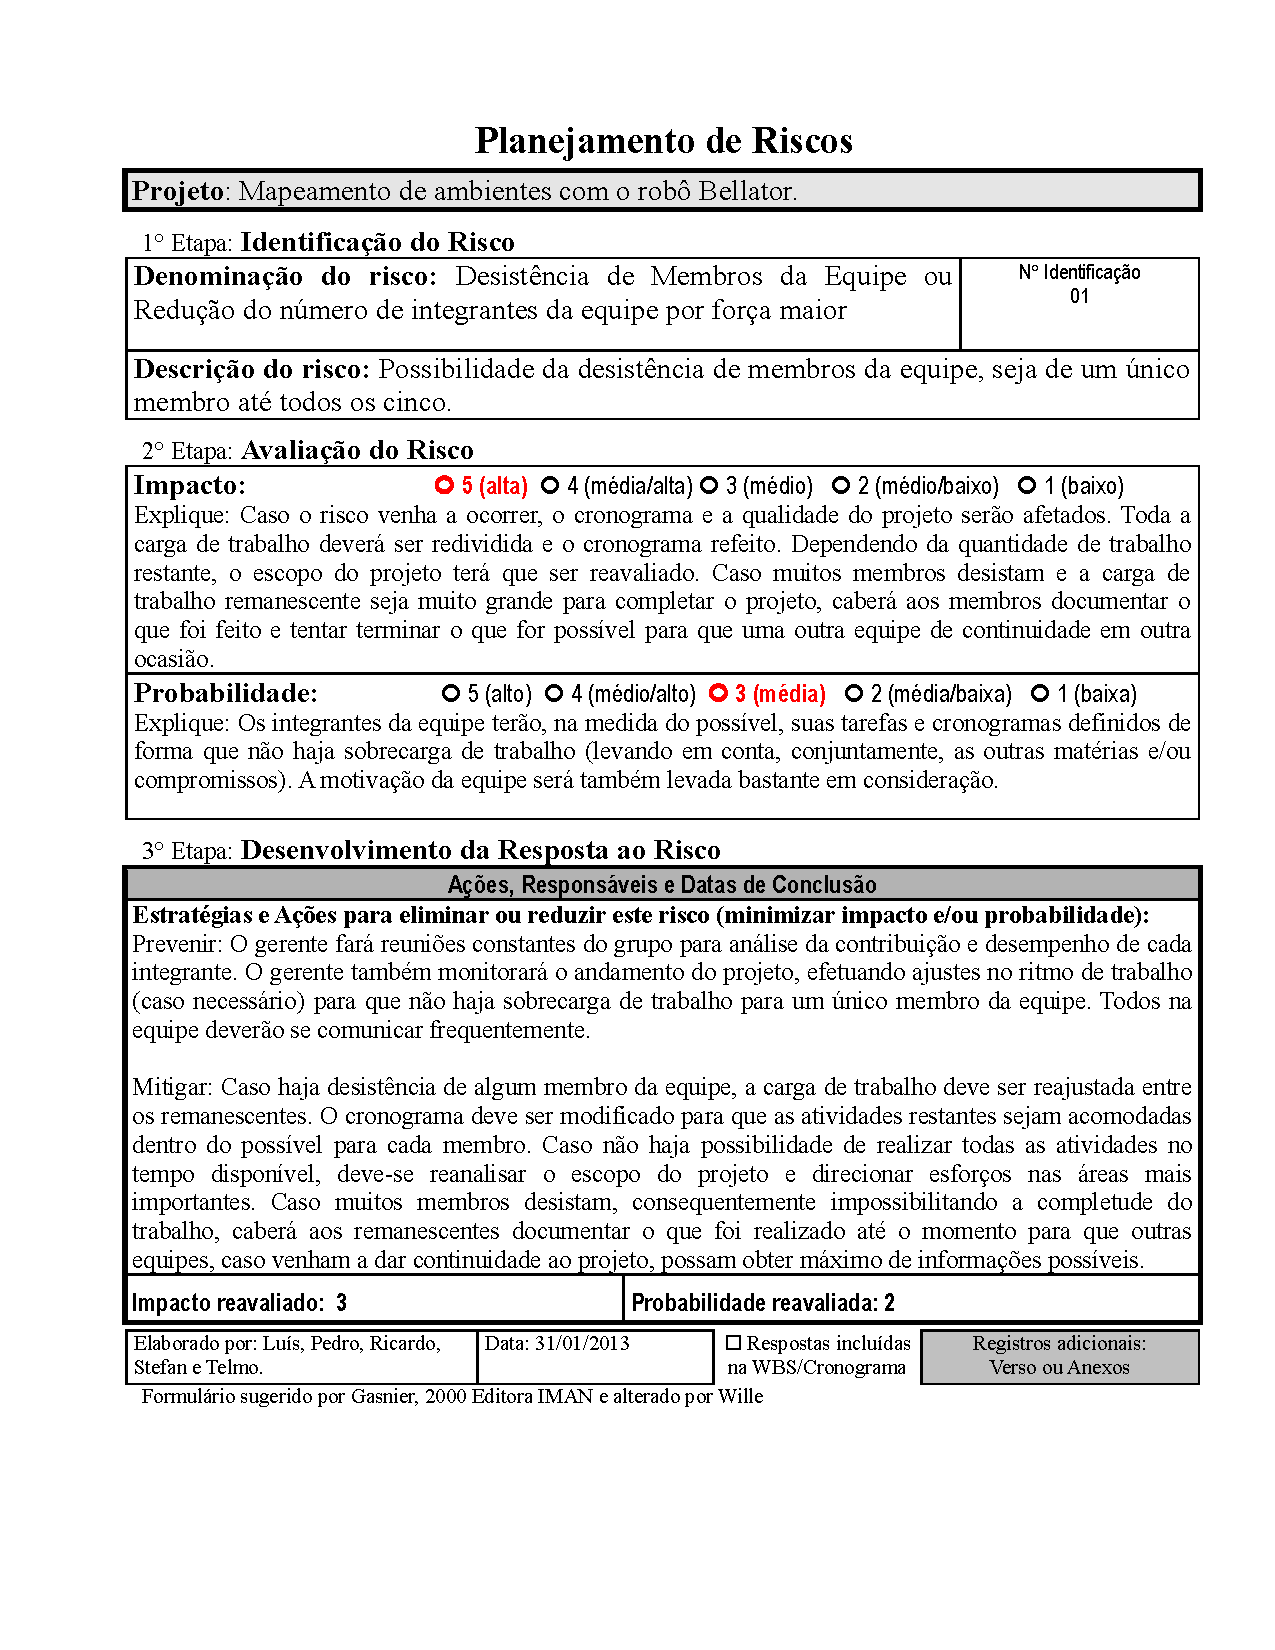
\includepdf[pages=1,scale=0.5, pagecommand=\chapter{Planejamento de riscos}]{Planejamento_de_Riscos_v3.pdf}
\includepdf[pages=2-9, pagecommand=]{Planejamento_de_Riscos_v3.pdf}

\chapter{Trabalhos correlatos}

O mapeamento de ambientes realizado por robôs visa ao desenvolvimento de software e hardware que permitam a construção de um mapa a partir de dados captados por um ou mais sensores. Há diversas tecnologias que podem ser empregadas para alcançar tal objetivo, como o processamento de digital de imagens captadas de uma câmera ou a utilização de sensores de proximidade tais como sensores de ultrassom ou sensores de ondas eletromagnéticas.

Esta última opção mostra-se bastante adequada para a maioria dos projetos, pois garante uma medição satisfatória da distância de objetos próximos ao robô a um custo não muito elevado. Um dos sensores mais populares deste tipo é o sensor de proximidade de infravermelho. Quando integrado ao robô permite a obtenção várias medidas discretas da distância do robô a objetos, um dos elementos básicos que permitem a geração do mapa do ambiente.

\subsection{PatrolBot}
O PatrolBot \cite{patrol_bot} é um robô configurável desenvolvido com interesses comerciais. Ele pode criar uma planta do interior de construções. Utilizando a tecnologia WI-FI ele pode ser controlado remotamente ou se movimentar de forma autônoma, sendo apenas monitorado pela estação base. Tal comunicação é feita por Wi-Fi.

Ele permite a inclusão de acessórios adicionais tais como uma câmera e microfones que permitirão ver e ouvir o que se passa no ambiente que está sendo mapeado. Há diversos outros periféricos que podem ser incluídos no robô, que também oferece a opção de ser programado, por meio de um kit de desenvolvimento próprio.

\subsection{Sistema de mapeamento robótico bidimensional por infravermelho}

Nesta implementação \cite{wii}, um telêmetro infravermelho é utilizado para obter a distância de objetos próximos. A câmera infravermelha do Nintendo Wii é utilizada juntamente com sinalizadores (LEDs) para triangular a posição do robô e sua direção.

Como hardware, foram utilizados: um Arduino Mini Pro, um cartão microSD, telêmetro inframervelho, câmera do Wii. Não há comunicação em tempo real com a estação base. Isto significa que os dados são obtidos e armazenados no cartão microSD. Para leitura, o cartão deve ser inserido em um computador e, então, carregado na estação base. Os resultados são visualizados em um arquivo textual simples, no qual a letra "O" simboliza a posição do robô e a letra "X" os obtáculos detectados.

\chapter{Análise tecnológica}
Nesta seção está explicitada, primeiramente, uma visão geral do projeto. Em seguida, há uma discussão detalhada a respeito dos requisitos de cada parte fundamental -- estação base, sistema de comunicação e sistema embarcado. Por fim há uma enumeração das alternativas tecnológicas pesquisadas e das escolhidas para o preenchimento dos requisitos.

\section{Visão geral do projeto}

O projeto, de um ponto de vista geral, consiste em um robô controlado manualmente e que seja capaz de efetuar mapeamento em duas dimensões de ambientes. Um usuário humano monitorará e controlará um computador -- a estação base -- a partir do qual poderão ser enviados comandos de movimentação, via teclado, ao robô. Informações sobre o posicionamento do robô e dos obstáculos detectados por ele serão recebidas na estação base em tempo real. Imagens instantâneas de uma câmera posicionada no robô -- aspecto explicado mais à frente -- poderão ser visualizadas pelo utilizador.

O sistema de comunicação deverá ter, ao menos, alcance de 20 metros sem fios. Visto que toda a comunicação entre a estação base e o sistema embarcado será feita por um único canal, a velocidade e o tipo de fluxo de transmissão de dados devem ser adequados para, simultaneamente, o envio de comandos de movimentação ao robô, recebimento de dados de leituras de sensores e recebimento de imagens da câmera.

O sistema embarcado é constituído, em suma, pelo robô. Ele deve ser capaz de se mover para frente e para trás e girar para a esquerda e direita. A visualização em tempo real do ambiente pelo utilizador, com o objetivo de facilitar o controle de movimentação manual, poderá ser feita através de imagens instantâneas geradas por uma câmera fixa instalada no robô. 

O robô deve ser capaz de obter dados para cálculos (na estação base) de sua velocidade e deslocamento. Um aspecto desejável em relação a isso é a atenuação de erros em decorrência de escorregamento, giros em falso ou trepidação de rodas, visando, dessa forma, a utilização futura do robô em condições não ideais de terreno. Obstáculos próximos -- em uma distância mínima de 30 cm e máxima de 150 cm -- devem ser detectados de modo a possibilitar a confecção de um mapa 2D em tempo real na estação base.

\section{Requisitos}


\subsection{Estação base}
%
%TODO verificar objetivos do projeto
Esta seção descreve os requisitos da estação base, que foram elaborados de forma a satisfazer os objetivos do projeto.

\begin{itemize} %-------------------

  \item O \textit{software} será executado em um computador pessoal.
    \begin{itemize}
%      \item O computador deverá possuir recursos de \textit{hardware} comparável aos padrões atuais (pelo menos 2GB de memória RAM DDR2 ou melhor e processador \textit{dual-core}).
      \item O \textit{software} deverá ser multiplataforma, ou seja, executar em diferentes sistemas operacionais (ao menos Linux e Windows).
      \item Preferencialmente bibliotecas e ferramentas livres (e gratuitas) deverão ser utilizadas no desenvolvimento do \textit{software}.
    \end{itemize}

  \item O software deve possuir uma interface gráfica.
    \begin{itemize}
      \item Um utilizador, através da interface gráfica, será capaz de controlar o robô enviando comandos de movimentação (especificados pelo teclado). 
      \item O usuário receberá a imagem em tempo real (preferencialmente com atrasos não muito consideráveis) de uma câmera fixa instalada no robô. 
      \item Os dados instantâneos de velocidade e posição do robô serão mostrados ao usuário na interface gráfica.
      \item Um mapa 2D do caminho percorrido e dos obstáculos detectados pelo robô será gerado, na interface gráfica, à medida em que o robô se movimentar. O caminho percorrido por ele será representado por pontos interpolados que demonstrem visulamente a trilha percorrida por ele. Os obstáculos serão representados por pontos, não interpolados, nos quais houve detecção de objetos pelos sensores. Todos os pontos representados no mapa serão gerados a partir de amostras em intervalos de tempo discretos de leituras de sensores do robô.
      \item O mapa 2D gerado na interface poderá ser salvo em um arquivo, podendo ser posteriormente carregado.
    \end{itemize}

\end{itemize} %----------------------



\subsection{Sistema de comunicação}
Esta seção descreve os requisitos do sistema de comunicação entre a estação base e o sistema embarcado.

\begin{itemize} %----------------------

  \item Distância entre robô e estação base.
    \begin{itemize}
      \item O sistema de comunicação deve possuir alcance máximo de 20 metros, de modo que ambientes de tamanho razoável possam ser mapeados.
    \end{itemize}

  \item Velocidade e direção do fluxo de transmissão de dados.
    \begin{itemize}
      \item A velocidade de transmissão do canal de comunicação deve ser suficiente para o envio de comandos de movimentação ao robô, recebimento de dados de leituras de sensores e recebimento de imagens da câmera em tempo real -- visto que toda a comunicação entre a estação base e o sistema embarcado será feita por um único canal.
      \item O fluxo de dados deve ser bidirecional (\textit{full-duplex}).
    \end{itemize}

\end{itemize} %----------------------



\subsection{Sistema embarcado}
Esta seção descreve os requisitos do sistema embarcado (robô).

\begin{itemize} %----------------------

  \item Movimentação do robô.
    \begin{itemize}
      \item O robô deve ser capaz de mover-se para frente, para trás e girar para a esquerda e direita em velocidades baixas.
%      \item A velocidade de movimentação pode ser relativamente pequena. %%TODO verificar velocidade do bellator nas monografias anteriores
    \end{itemize}

  \item Controle de posicionamento e velocidade.
    \begin{itemize}
      \item O robô deve ser capaz de obter dados que permitam calcular sua velocidade (linear e angular) e posição (deslocamento e rotação), enviando-os à estação base.
    \end{itemize}

  \item Detecção de obstáculos.
    \begin{itemize}
      \item O robô deverá ser capaz de detectar obstáculos próximos -- com distância de no mínimo 30 cm e no máximo 150 cm -- localizados ao seu redor, determinando a distância de cada objeto detectado.
    \end{itemize}

\end{itemize} %----------------------


\section{Análise de opções tecnológicas}

Nesta seção está apresentada a análise das opções tecnológicas plausíveis para o atendimento dos requisitos. As alternativas pesquisadas e as escolhidas para cada parte do projeto estão explicitadas a seguir.

\subsection{Estação base}

As alternativas pesquisadas para a estação base estão apresentadas nesta subseção.

\subsubsection{Biblioteca para desenhos 2D}
\label{subsec:alternativas_desenho}

Tendo em vista que um dos requisitos é a geração de um mapa em duas dimensões na estação base, deve-se escolher uma biblioteca que permita realizar o desenho de formas geométricas diversas e que possa ser integrada facilmente à interface gráfica. Ela deve também possuir meios simples de obter informações do mouse e teclado, para interatividade com o usuário. 

Uma biblioteca interessante disponível em Java que possui o recurso de produzir desenhos dinâmicos (e integrá-los a interfaces gráficas) é o Processing \cite{processing}, \textit{open-source}. Essa biblioteca foi a principal encontrada que seria capaz de satisfazer as necessidades de desenho do mapa 2D de forma simples. Por possuir inúmeras funções de desenho em alto nível, o trabalho de renderização dos gráficos seria consideravelmente simplificado. Além disso, na biblioteca existem recursos que permitem o recebimento de informações de posicionamento do mouse e de comandos do teclado. Por ser constituído basicamente de um \textit{Applet} Java, o Processing pode facilmente ser integrado a componentes do Swing -- biblioteca de interface gráfica (GUI) do Java.


Outra biblioteca para a confecção de desenhos em 2D é o Cairo \cite{cairo}, que é \textit{open-source}, disponível nas linguagens C e C++. Ele possui recursos em alto nível para renderização de formas e interação com o usuário, assim como o Processing. Nos aspectos gerais as duas ferramentas são muito semelhantes. A integração do Cairo com a interface gráfica, porém, é dependente na biblioteca externa de GUI utilizada para tal.

Um aspecto importante a notar é que ambas as bibliotecas foram desenvolvidas e otimizadas para terem bom desempenho em máquinas atuais -- o que é desejável tendo em vista os requisitos. Na Tabela \ref{tab:alternativas_desenho} está presente uma comparação entre as duas bibliotecas.


\begin{table}[h]
  \caption{Comparação entre Bibliotecas para desenhos 2D.}
  \centering
  \begin{tabular}{p{6cm}|p{4cm}p{4cm}}
    \toprule
    \textbf{Característica} & \textbf{Cairo} & \textbf{Processing} \\
    \midrule
    Linguagem de programação & C e C++ & Java \\
    \hline
    Integração com interface gráfica & Sim (depende da biblioteca de GUI utilizada) & Sim (na biblioteca Swing do Java) \\
    \hline
    Ferramentas de interação com o usuário & Sim & Sim \\
    \bottomrule
  \end{tabular}
  \label{tab:alternativas_desenho}
\end{table}

A escolha da biblioteca de desenhos foi feita em conjunto com a escolha de linguagem de programação. A biblioteca escolhida, dentre as duas opções, foi o Processing, visto que a integração a interfaces gráficas do Java é muito simples. 

\subsubsection{Linguagem de programação}

Nessa etapa de avaliação das opções, a escolha de uma boa linguagem de programação que atenda aos requisitos é fundamental. Abaixo está presente uma lista dos aspectos desejáveis da linguagem:

\begin{itemize}
  \item Deve ser multiplataforma (ao menos compatível com Linux e Windows sem muitas modificações);
  \item Deve possuir orientação a objetos;
  \item Deve possuir recursos multiplataforma e \textit{open-source} para o desenvolvimento de interfaces gráficas;
  \item Deve ter a disponibilidade de ferramentas \textit{open-source} e multiplataforma para a criação visual da interface gráfica, dessa forma agilizando o processo de desenvolvimento;
  \item Deve possuir recursos, integrados ou em bibliotecas \textit{open-source}, para o desenvolvimento de desenhos dinâmicos (para a geração do mapa 2D). Os desenhos devem ser facilmente integráveis à interface gráfica.
\end{itemize}


Abaixo está presente uma descrição das duas linguagens, o C++ e Java, atualmente utilizadas em inúmeras aplicações, e que são potenciais alternativas ao projeto. A Tabela \ref{tab:alternativas_linguagens} sumariza os recursos de cada uma.

\textbf{Java}

O Java \cite{java} é uma linguagem concebida de início como sendo orientada a objetos. A maneira com que é feita a compilação e execução do código permite que muito facilmente programas sejam rodados em diferentes plataformas (Linux, Windows, Mac, entre outros). O processo de compilação do código gera os chamados \textit{bytecodes}, que são instruções a serem interpretadas pela \textit{Java Virtual Machine} (JVM). A grande vantagem é que o JVM possui disponibilidade multiplataforma, e a manutenção pelos desenvolvedores é frequente.

Há disponibilidade, na API do Java, da biblioteca Swing -- que contém recursos completos para a criação de interfaces gráficas (GUI) interativas. Existem ferramentas visuais de código aberto que consideravelmente agilizam o processo de desenvolvimento de interfaces Swing, entre elas o NetBeans \cite{netbeans} e o Eclipse \cite{eclipse}, através de plugins ou extensões. 

Para o preenchimento do requisito de confecção de desenhos em 2D com integração à interface gráfica, a biblioteca do Processing (explicada anteriormente na Subseção \ref{subsec:alternativas_desenho}) está disponível nessa linguagem.


\textbf{C++}

O C++ é uma linguagem orientada a objetos, que foi desenvolvida a partir da linguagem C. A compilação de código no C++ deve ser feita especificamente para cada plataforma em que os programas desenvolvidos forem utilizados. De uma perspectiva prática, certas seções de código frequentemente necessitam de adaptações manuais para cada plataforma e sistema operacional, o que gera retrabalho e gastos de tempo adicionais. 

Recursos para desenvolvimento visual de interfaces gráficas estão disponíveis através de bibliotecas e ferramentas externas. O C++ não possui recursos de interface gráfica na própria API. Deve-se notar que esse é um aspecto que adiciona complexidade ao portar programas entre diferentes sistemas. 

Para a confecção de desenhos 2D e incorporação dos mesmos à interface gráfica, a biblioteca Cairo (explicada anteriormente na Subseção \ref{subsec:alternativas_desenho}) pode ser utilizada com essa linguagem. A possibilidade de haver integração com a interface, porém, é dependente da biblioteca de GUI utilizada.


\textbf{Escolha da equipe:} O Java foi a linguagem escolhida para o desenvolvimento do \textit{software} da estação base, uma vez que preenche satisfatoriamente os requisitos do projeto. A escolha do Java foi feita em conjunto com a escolha da biblioteca do Processing. Notavelmente, há a facilidade em portar, sem adaptações, programas para diferentes plataformas, processo este que é mais complexo no C++.  Com relação ao quesito de desempenho em computadores atuais, a linguagem escolhida é satisfatória, visto que há manutenção constante da implementação das bibliotecas e da máquina virtual do Java pelos desenvolvedores -- que buscam, entre outros aspectos, otimizar a linguagem para tecnologias atuais.

\begin{table}[h]
  \caption{Comparação entre linguagens de programação.}
  \centering
  \begin{tabular}{p{6cm}|p{4cm}p{4cm}}
    \toprule
    \textbf{Característica} & \textbf{C++} & \textbf{Java} \\
    \hline
    Multiplataforma (Linux e Windows) & Sim (com adaptação) & Sim (sem adaptação) \\
    \hline
    Orientação a objetos & Sim & Sim \\
    \hline
    Recursos multi-plataforma e \textit{open-source} para desenvolvimento de interface gráfica (GUI) & Sim (com bibliotecas externas) & Sim (integrado à API da linguagem) \\
    \hline
    Ferramentas \textit{open-source} e multiplataforma para criação visual de interface gráfica & Sim (ferramentas externas) & Sim (ferramentas externas) \\
    \hline
    Recursos \textit{open-source} para desenvolvimento de desenhos dinâmicos, facilmente integráveis à interface gráfica & Sim (biblitoeca externa, integração à interface gráfica dependente da GUI utilizada) & Sim (biblioteca externa) \\
    \bottomrule
  \end{tabular}
  \label{tab:alternativas_linguagens}
\end{table}



\subsection{Sistema de comunicação}

Na Tabela \ref{tab:alternativas_comunicacao} está presente uma comparação entre diferentes tecnologias de comunicação sem fios. O Wi-Fi é o recurso mais atrativo em todos os aspectos que foram comparados, preenchendo satisfatoriamente os requisitos do sistema de comunicação. Sua velocidade e alcance são suficientes para satisfazer as necessidades, e o fluxo de dados pode ser \textit{full-duplex}. Notavelmente, o Wi-Fi é o único sistema comparado que oferece a possibilidade (com simplicidade) de uso do protocolo TCP -- o que é um requisito importante para o desenvolvimento ágil e satisfatório do projeto.


\begin{table}[h]
  \caption{Comparação entre tecnologias de comunicação sem fios.}
  \centering
  \begin{tabular}{p{4.5cm}|p{3cm}p{4cm}p{2cm}}
    \toprule
    \textbf{Característica} & \textbf{802.11g (Wi-Fi)} & \multicolumn{1}{l}{\textbf{Rádio Frequência (RF)}} & \textbf{Bluetooth}  \\
    \hline
    Distância máxima de alcance & 50-100 metros  & 30-100 metros & 10 metros \\
    \hline
    Velocidade de transmissão máxima & 54 Mbits/s & 2 Mbits/s & 1 Mbits/s \\
    \hline
    Fluxo de dados \textit{full-duplex} & Sim & Sim & Sim \\
    \hline
    Possibilidade e simplicidade de uso de TCP & Sim & Não & Não \\
    \bottomrule
  \end{tabular}
  \label{tab:alternativas_comunicacao}
\end{table}



\subsection{Sistema embarcado}

Nesta seção apresentamos as alternativas pesquisadas para o sistema embarcado, levando em conta os requisitos já apresentados anteriormente.

\subsubsection{Movimentação do robô}

O sistema de movimentação do robô, incluindo motores, acionadores, drivers de potência e rodas não foram pesquisados pois já estão implementados no robô e atendem aos requisitos especificados nas seções anteriores. Sendo assim utilizaremos um chassi de 40 cm de largura por 50 cm de comprimento, duas rodas de tração e uma roda guia. As rodas de tração estão dispostas na parte posterior do robô, possuindo 20 cm de diâmetro e 4 cm de largura. O chassi está equipado com 2 motores Bosch FPG 12V, 2 baterias Unybatt 12V-7,2 Ampére-hora e duas pontes H L298 \cite{bellator_2012}. A disposição dos itens no robô pode ser vista na figura \ref{fig:disposicao_bellator_2012}.

\begin{figure}[H]
\centering
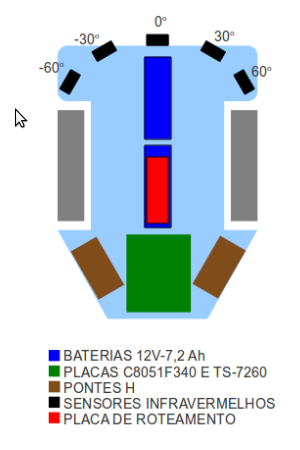
\includegraphics[width=0.4\textwidth]{./figuras/disposicao-robo.png}
\caption[Disposição dos itens no robô]{Disposição dos itens no robô}
\fonte{\cite{bellator_2012}}
\label{fig:disposicao_bellator_2012}
\end{figure}

\subsubsection{Odometria}

Para a obtenção da direção e sentido do movimento do robô, assim como aceleração, velocidade e posição, pode-se optar por diversos tipos de tecnologias ou pela associação delas. Abaixo descrevemos as principais delas.

\begin{itemize}
  \item \textbf{Encoder:} Ligado ao eixo da roda do robô, conta a quantidade de voltas dadas pela roda. Permite assim calcular a distancia percorrida pelo robô. Caso sejam conectados dois encoders, um em cada roda, podemos obter também a direção do movimento pela diferença entre a contagem de voltas de cada roda.
  \item \textbf{GPS:} Utiliza sinais de satélites para obter as coordenadas geográficas do robô. A direção e o sentido podem ser obtidos pela comparação das leituras com as anteriores.
  \item 	\textbf{Acelerômetro:} pode utilizar a tecnologia chamada \textbf{MEMS} para medir a aceleração sofrida pelo componente.
  \item 	\textbf{Giroscópio:} pode utilizar a tecnologia chamada \textbf{MEMS} para medir a aceleração angular sofrida pelo componente.
  \item 	\textbf{Bussola:} Utiliza os campos magnéticos da terra para obter a direção com relação aos polos magnéticos da terra.
\end{itemize}

A seguir, na tabela \ref{tab:alternativas_tecnologias_odometria}, comparamos as tecnologias apresentadas anteriormente. 

\begin{table}[h]
  \caption{Comparação entre tecnologias para odometria.}
  \centering
  \begin{tabular}{p{3cm}|p{2.2cm}p{1.7cm}p{2.2cm}p{2.2cm}p{2.2cm}}
    \toprule
    \textbf{Característica} & \textbf{Encoder} & \textbf{GPS} & \textbf{Acelerômetro} & \textbf{Giroscópio} & \textbf{Bussola} \\
    \hline
    Sujeito a influencias externas & Deslizamentos & Não & Não & Não & Campo magnético dos motores \\
    \hline
    Ambiente de operação & Interno / Externo & Externo & Interno / Externo & Interno / Externo & Interno / Externo \\
    \hline
    Posicionamento & Relativo & Absoluto & Relativo & Relativo & Relativo \\
    \bottomrule
  \end{tabular}
  \label{tab:alternativas_tecnologias_odometria}
\end{table}

Com base no comparativo da tabela \ref{tab:alternativas_tecnologias_odometria} optamos por utilizar um acelerômetro em conjunto com um giroscópio para obter os dados para odometria. Encoders estão sujeitos a erros causados por deslizamento nas rodas, GPS apenas funciona em ambientes externos e a bussola pode ser influenciada pelo campo magnético dos motores. Como o robô já apresenta encoders instalado, utilizaremos também os dois encoders, possibilitando assim aumentar a precisão e confiabilidade dos dados de odometrias.
Justificada nossa escolha por acelerômetros e giroscópios, na tabela \ref{tab:alternativas_componentes_odometria} fazemos um comparativo entre as opções de menor custo disponíveis no mercado. Listamos na tabela apenas as alternativas que possuem placas de desenvolvimento pois acelerômetros e giroscópios são geralmente são vendidos em encapsulamento LGA, os quais são de difícil soldagem.

\begin{table}[h]
  \caption{Comparação entre acelerômetros/giroscópios para odometria.}
  \centering
  \begin{tabular}{p{2.4cm}|p{3cm}p{0.8cm}p{1.4cm}p{1.8cm}p{1.7cm}p{1.3cm}}
    \toprule
    \textbf{Modelo} & \textbf{Fabricante} & \textbf{Acel.} & \textbf{Giro.} & \textbf{Faixa} & \textbf{Interface} & \textbf{Preço} \\
    \hline
    STEVAL-MKI009V1	& STMicroeletronics & 3x	& - & $ \pm 2g / \pm6g $ & I2c / SPI & \$23.94 \\
    \hline
	ATAVRSBIN1 & Atmel & 1x & - & - & I2c & \$26.25 \\
	\hline
	KIT3803 MMA7660FC & Freescale & 3x & - & $ \pm 1.5g $ & I2C & 	\$35.0 \\
	\hline
	ATAVRSBIN1 & Atmel & - & 1x & & I2C & \$26.25 \\
	\hline
	MPU-6050	 & IvenSense & 3x & 3x & $ \pm 2g / \pm 4g $ $ \pm 250 ^{o}/seg /$ $ \pm 500 ^{o}/seg $ & I2C & \$8.78 \\
    \hline
	MKI086V1	 & STMicroeletronics & 1x & $ \pm 30^{o}/seg $ & Analog & & \$31.50 \\
	\hline
	STEVAL-MKI094V1 & STMicroeletronics & - & 3x & $ \pm 400^{o}/seg $ & Analog & \$31.50 \\
	\hline
	ATAVRSBIN1 & Atmel & 1x & 1x & & I2C & \$26.25 \\
	\hline
	DM240316	 & Zena & 3x & 3x & 	& RF & \$99.99 \\
    \bottomrule
  \end{tabular}
  \label{tab:alternativas_componentes_odometria}
\end{table}

\textbf{MPU-6050}

Com base na tabela \ref{tab:alternativas_componentes_odometria} escolhemos o modelo MPU-6050 da IvenSense principalmente devido ao seu baixo custo: \$8.78. Este modelo possui um acelerômetro de 3 eixos, um giroscópio e 3 eixos e entradas para uma bussola externa integrados em um único chip \cite{mpu6050}. A faixa de operação para o acelerômetro é de $ \pm 2g ou \pm 4g $ e para o giroscópio é de $ \pm 250 ^{o}/seg $ ou $ \pm 500 ^{o}/seg $. A sensibilidade do acelerômetro é de $ 16384 LSB/g $ e $ 8192 LSB/g $. A sensibilidade do giroscópio é de $ 131 LSB/ ^{o} / seg $ e $ 65.5 LSB/ ^{o} / seg $. A interface de comunicação do módulo suporta o protocolo I2C. O módulo contendo o chip MPU-6050 e alguns componentes necessários para seu funcionamento pode ser visto na figura \ref{fig:mpu6050}.

\begin{figure}[H]
\centering
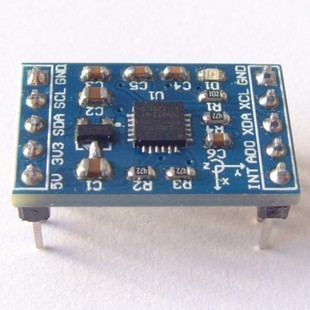
\includegraphics[width=0.4\textwidth]{./figuras/mpu6050.JPG}
\caption[Placa de desenvolvimento contendo o chip MPU-6050]{Placa de desenvolvimento contendo o chip MPU-6050}
\fonte{\cite{mpu6050}}
\label{fig:mpu6050}
\end{figure}

\textbf{Encoder Optico HEDS-9700}

Como já foi dito, utilizaremos também os encoders já existentes no robô. O robô está equipado com dois encoders HEDS-9700.
Esses encoders geram em sua saída uma onda quadrada à medida em que o encoder é rotacionado, sendo 1800 pulsos gerados em uma rotação \cite{heds9700}. A forma de onda da saída do encoder pode ser vista na figura \ref{fig:heds9700}. Podemos ver na figura que o encoder possui duas saidas, A e B com defasamento $\phi$ entre elas. Com as duas saídas podemos determinar o sentido de rotação. Porém na implementação existente esse recurso não é utilizado.

\begin{figure}[H]
\centering
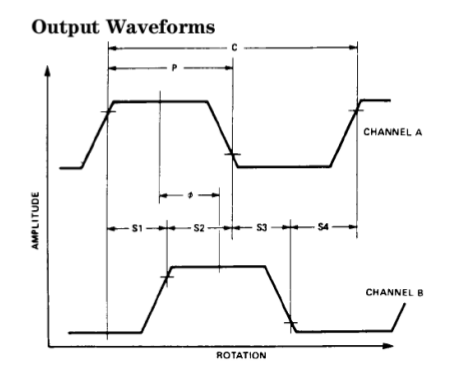
\includegraphics[width=0.6\textwidth]{./figuras/heds9700.png}
\caption[Forma de onda de saída do encoder]{Forma de onda de saída do encoder}
\fonte{\cite{heds9700}}
\label{fig:heds9700}
\end{figure}

\subsubsection{Detecção de obstáculos}

\textbf{Sensor de proximidade Infra Vermelho IR 2Y0A02F98}

A detecção de obstáculos, que é um requisito deste robô, será atendido pelos sensores de Infra vermelho já existentes no robô. Logo serão utilizados sensores IR 2Y0A02F98 \cite{ir_sensor}. Este modelo é pouco influenciado pelas cores dos objetos detectados devido ao método de medição baseado em triangulação. Na figura \ref{fig:ir_sensor_response} podemos ver isso. A linha tracejada é a resposta para reflexão em um papel cinza e a linha contínua é a resposta para reflexão em um papel branco.

\begin{figure}[H]
\centering
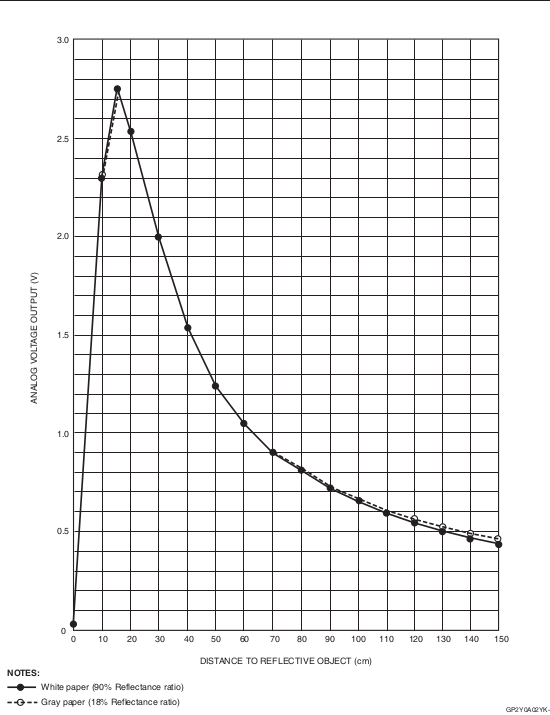
\includegraphics[width=1\textwidth]{./figuras/ir-sensor-response.png}
\caption[Curva de resposta do encoder]{Curva de resposta do encoder}
\fonte{\cite{ir_sensor}}
\label{fig:ir_sensor_response}
\end{figure}

\subsubsection{Microcontrolador}

A interface entre os sensores, atuadores e a placa TS-7260 já existente no robô \cite{bellator_2012} será feita por um sistema micro controlado. Uma vez escolhidos os sensores, o sistema micro controlado deve possuir as interfaces adequadas para comunicação com os sensores e também para comunicação com o hardware já existente no robô, como o sistema de acionamento dos motores e interface com a placa TS-7260. Desta forma, na tabela \ref{tab:requisitos_microcontrolador} listamos os requisitos para escolha do microcontrolador. Na tabela \ref{tab:requisitos_desejaveis_microcontrolador} listamos os requisitos que não são obrigatórios, porém desejáveis para o microcontrolador.

\begin{table}[h]
  \caption{Requisitos para escolha do microcontrolador.}
  \centering
  \begin{tabular}{p{7cm}|p{8cm}}
    \toprule
    \textbf{Requisito} & \textbf{Justificativa} \\
    \hline
    Interface I2C & Comunicação com acelerômetro e giroscópio \\
    \hline
    Geração de PWM em 4 canais & Acionamento dos motores pelas pontes H \\
    \hline
    Interface Serial	 & Comunicação com a placa TS-7260 \\
    \hline
    Interrupções em 2 canais	 & Leitura do valor dos encoders \\
    \hline
    Conversor AD em 5 canais	 & Leitura dos sensores de IR \\
    \bottomrule
  \end{tabular}
  \label{tab:requisitos_microcontrolador}
\end{table}

\begin{table}[h]
  \caption{Requisitos desejáveis para escolha do microcontrolador.}
  \centering
  \begin{tabular}{p{7cm}|p{8cm}}
    \toprule
    \textbf{Requisito desejável} & \textbf{Justificativa} \\
    \hline
    Desenvolvimento em plataforma livre	 & Diminui o custo de softwares para desenvolvimento \\
    \hline
    32 bits & Facilita manipulações numéricas na programação, diminuindo esforço e custo para programação \\
    \hline
    2 Interfaces seriais ou JTAG & Utilização para debug ou logs \\
    \hline
    Solução integrada & Redução do tamanho da placa e quantidade de componentes, diminuindo assim o custo e melhorando a organização e disposição dos componentes \\
    \bottomrule
  \end{tabular}
  \label{tab:requisitos_desejaveis_microcontrolador}
\end{table}

Na tabela \ref{tab:alternativas_microcontrolador} listamos diversas opções de microcontroladores que foram pesquisados para o projeto. Todas as opções atendem aos requisitos da tabela \ref{tab:requisitos_microcontrolador}, e são 32 bits.

\begin{table}[h]
\caption{Comparativo entre microcontroladores.}
\fonte{Dados obtidos de \cite{digikey}}
\centering
\begin{tabular}{l|rrrrrr}
\toprule
\textbf{uC} & \textbf{STM32F103C6T7A} & \textbf{PIC32MX320F128H} & \textbf{LPC2103} \\ \hline
Fabricante & STMicroelectronics & Microchip Technology & NXP Semiconductors \\ \hline
Arquitetura & ARM® Cortex™-M3 & MIPS32® M4K™ & ARM7 \\ \hline
Core & 32bits & 32-Bit & 16/32-Bit \\ \hline
Velocidade & 72MHz & 80MHz & 70MHz \\ \hline
MIPS & 90 & 124.8 & 63 \\ \hline
I2C & 1 & 2 & 2 \\ \hline
PWM & 12 & 5 & 14 \\ \hline
UART & 2 & 2 & 2 \\ \hline
Einterrupt & 16 & 5 & 13 \\ \hline
FLASH & 32k & 128k & 32k \\ \hline
RAM & 10k & 16k & 8k \\ \hline
Adc & 10x12b & 16x10b & 8x10b \\ \hline
JTAG & sim & sim & sim \\ \hline
Custo & \$6.27 & \$6.26 & \$6.16 \\
\toprule
\textbf{uC} & \textbf{MCF52210CAE66} & \textbf{AT32UC3C264C} & \textbf{SIM3C146} \\ \hline
Fabricante & Freescale Semiconductor & Atmel & Silicon Laboratories Inc \\ \hline
Arquitetura & Coldfire V2 & AVR & ARM® Cortex™-M3 \\ \hline
Core & 32-Bit & 32-Bit & 32-Bit \\ \hline
Velocidade & 66MHz & 66MHz & 80MHz \\ \hline
MIPS & 75.9 & 98.34 & 100 \\ \hline
I2C & 2 & 3 & 2 \\ \hline
PWM & 4 & 8 & 8 \\ \hline
UART & 3 & 1 & 2 \\ \hline
Einterrupt & 7 & 7 & 16 \\ \hline
FLASH & 64k & 64k & 64k \\ \hline
RAM & 16k & 16k & 16k \\ \hline
Adc & 8x12b & 11x12b & 28x12b \\ \hline
JTAG & sim & sim & SIM3C146-B-GQ \\ \hline
Custo & \$7.1 & \$9.14 & \$6.1 \\ \bottomrule
\end{tabular}
\label{tab:alternativas_microcontrolador}
\end{table}

Dentre as opções listadas na tabela \ref{tab:alternativas_microcontrolador} escolhemos a opção \textbf{LPC2103}. Esta escolha foi feita baseada principalmente no custo do microcontrolador. Porém ao compará-lo com o \textbf{SIM3C146} vemos que esta última opção possui desempenho melhor com custo menor. Nossa escolha pelo \textbf{LPC2103} e não pelo \textbf{SIM3C146} justifica-se pela melhor documentação e disponibilidade de recursos para o \textbf{LPC2103}. A documentação fornecida pelo fabricante do microcontrolador \textbf{LPC2103} é mais completa, e por já estar a mais tempo no mercado a quantidade de informações e recursos disponíveis na internet é maior.

\textbf{LCP2103}

O \textbf{LCP2103} é um microcontrolador baseado na arquitetura ARM7TDMI-S da NXP \cite{lpc2103}. Este microcontrolador pode operar em até $ 70MHz $ executando a $ 63MIPS $. O Microcontrolador possui 2 interfaces I2C, 2 interfaces seriais, até 14 saídas de PWM, até 13 canais de interrupções externas, 8 canais de conversão para um conversor analógico digital de 10 bits, 32kbytes de memória FLASH para código e 8kbytes de memória RAM. Ele também suporta \textit{debug} via JTag por meio de um \textit{debugger} JTag externo. O custo desse microcontrolador é de \$6.16 \cite{digikey}.

O microcontrolador escolhido também pode ser programado utilizando o protocolo ISP por meio de ferramentas livres como o lpc21isp \cite{lpc21isp}. Para geração do código hexadecimal utilizado pelo lpc21isp basta compilar o código em C utilizando o GCC \cite{gcc}.
Portanto o \textbf{LCP2103} além de atender aos requisitos propostos anteriormente também atende aos requisitos desejáveis que foram propostos na tabela \ref{tab:requisitos_desejaveis_microcontrolador}.


\chapter{Plano do projeto}
\section{Cronograma}
O cronograma do projeto está presente em anexo, em um arquivo do OpenProj denominado ``Bellator.pod''.

\section{Deliverables}

Na Tabela \ref{tab:deliverables1} estão expostos os \textit{deliverables} previstos ao longo do projeto.

\begin{table}[h]
  \centering
  \caption{Relação dos entregáveis com seus respectivos responsáveis e prazos}
  \begin{tabular}{|p{3cm}|p{4cm}|p{7cm}|}
    \toprule
    \textbf{Dia}   & \textbf{Auxiliar de Gerenciamento} & \textbf{Deliverables} \\
    \hline
    13/03/2013 & Stefan Campana Fuchs & 
    \begin{enumerate}[topsep=0pt, partopsep=0pt, itemsep=0pt]
      \item Versões iniciais dos diagramas de casos de uso e de classes (estação base).
      \item Versão inicial do diagrama em blocos (hardware).
      \item Explicação inicial de cada bloco (hardware).
    \end{enumerate}\\
    \hline
    27/03/2013 & Telmo Friesen & 
    \begin{enumerate}[topsep=0pt, partopsep=0pt, itemsep=0pt]
      \item Versão inicial do diagrama de casos de uso (software embarcado).
      \item Versão inicial do diagrama de fluxo de dados (software embarcado).
      \item Versão inicial dos diagramas de estados (sistema de comunicação).
      \item Versão inicial da descrição das mensagens e codificações dos comandos (sistema de comunicação).
      \item Versão inicial do diagrama elétrico/eletrônico (hardware).
    \end{enumerate}\\
  \end{tabular}%
  \label{tab:deliverables1}%
\end{table}%


\begin{table}[h]
  \centering
  \begin{tabular}{|p{3cm}|p{4cm}|p{7cm}|}
    10/04/2013 & Ricardo Farah & 
    \begin{enumerate}[topsep=0pt, partopsep=0pt, itemsep=0pt]
      \item Diagrama de casos de uso e de classes (estação base).
      \item Diagrama de casos de uso (software embarcado).
      \item Diagrama de fluxo de dados (software embarcado).
      \item Diagrama em blocos (hardware).
      \item Explicação detalhada de cada bloco (hardware).
      \item Diagrama elétrico/eletrônico (hardware).
    \end{enumerate}\\
    \hline
    24/04/2013 & Stefan Campana Fuchs & 
    \begin{enumerate}[topsep=0pt, partopsep=0pt, itemsep=0pt]
      \item Projeto da PCB (Printed Circuit Board) (hardware).
      \item Lista de componentes para confecção da PCB completa (hardware).
      \item Diagramas de estados (sistema de comunicação).
      \item Descrição das mensagens e codificações dos comandos (sistema de comunicação).
      \item Descrição do uso do Software (Manual do Usuário)
      \item Mapa de conexão da PCB com a alimentação e outros elementos (hardware).
      \item Guia de montagem (hardware).
    \end{enumerate}\\
    \bottomrule
  \end{tabular}%
  \label{tab:deliverables2}%
\end{table}%

\chapter{Or\c{c}amento Detalhado}

\begin{table}[!h]\tiny
  \centering
  \caption{Pre\c{c}o individual e total dos componentes do projeto}
    \begin{tabular}{rrccrr}
    \toprule
    \multicolumn{6}{c}{\textbf{Fornecedor: Digikey}} \\
    \multicolumn{1}{c}{\textbf{Item}} & \multicolumn{1}{c}{\textbf{Quantidade}} & \multicolumn{1}{c}{\textbf{Descri\c{c}\~ao}} & \multicolumn{1}{c}{\textbf{Descri\c{c}\~ao textual}} & \textbf{Preco unitário} & \textbf{Subtotal} \\
    \multicolumn{1}{c}{1} & \multicolumn{1}{c}{4} & \multicolumn{1}{c}{IC REG LDO 5V .95A SOT-223} & \multicolumn{1}{c}{REGULADOR 5V} & \$0,54 & \$2,16 \\
    \multicolumn{1}{c}{2} & \multicolumn{1}{c}{3} & \multicolumn{1}{c}{IC REG LDO 3.3V .95A SOT-223} & \multicolumn{1}{c}{REGULADOR 3V3} & \$0,54 & \$1,62 \\
    \multicolumn{1}{c}{3} & \multicolumn{1}{c}{4} & \multicolumn{1}{c}{IC REG LDO 1.8V .95A SOT-223} & \multicolumn{1}{c}{REGULADOR 1V8} & \$0,48 & \$1,92 \\
    \multicolumn{1}{c}{4} & \multicolumn{1}{c}{4} & \multicolumn{1}{c}{IC BUFF/DVR TRI-ST DUAL 20SOIC} & \multicolumn{1}{c}{BUFFER P/ PWM} & \$0,99 & \$3,96 \\
    \multicolumn{1}{c}{5} & \multicolumn{1}{c}{3} & \multicolumn{1}{c}{IC ARM7 MCU FLASH 32K 48-LQFP} & \multicolumn{1}{c}{LPC 2103} & \$6,16 & \$18,48 \\
    \multicolumn{1}{c}{6} & \multicolumn{1}{c}{3} & \multicolumn{1}{c}{IC BUFF/DVR SCHM TRG 6BIT 14SOIC} & \multicolumn{1}{c}{SCHMITT TRIGGER} & \$1,52 & \$4,56 \\
    \multicolumn{1}{c}{7} & \multicolumn{1}{c}{25} & \multicolumn{1}{c}{RES 47.0K OHM 1/8W 1\% 0805} & \multicolumn{1}{c}{RESISTOR PULL-UP 47K} & \$0,01 & \$0,23 \\
    \multicolumn{1}{c}{8} & \multicolumn{1}{c}{4} & \multicolumn{1}{c}{LED CHIPLED 645NM RED DIFF 0805} & \multicolumn{1}{c}{LED VERMELHO 1V8 20MA} & \$0,09 & \$0,36 \\
    \multicolumn{1}{c}{9} & \multicolumn{1}{c}{4} & \multicolumn{1}{c}{RES 20K OHM 1/8W 1\% 0805 SMD} & \multicolumn{1}{c}{RESISTOR LED 20K} & \$0,04 & \$0,16 \\
    \multicolumn{1}{c}{10} & \multicolumn{1}{c}{25} & \multicolumn{1}{c}{RES 22.0 OHM 1/8W 1\% 0805 SMD} & \multicolumn{1}{c}{22 OHMS P/ LIMITADOR DE VOLTAGEM} & \$0,01 & \$0,37 \\
    \multicolumn{1}{c}{11} & \multicolumn{1}{c}{12} & \multicolumn{1}{c}{DIODE ZENER DUAL 4.3V SOT-363} & \multicolumn{1}{c}{DUAL ZENER 4V3} & \$0,33 & \$4,01 \\
    \multicolumn{1}{c}{12} & \multicolumn{1}{c}{10} & \multicolumn{1}{c}{CAP CER 150PF 50V 1\% NP0 0805} & \multicolumn{1}{c}{CAPACITOR 150P FILTRO ENCODERS} & \$0,12 & \$1,24 \\
    \multicolumn{1}{c}{13} & \multicolumn{1}{c}{10} & \multicolumn{1}{c}{RES 332 OHM 1/8W 1\% 0805 SMD} & \multicolumn{1}{c}{RESISTOR 332 FILTRO ENCODERS} & \$0,02 & \$0,19 \\
    \multicolumn{1}{c}{14} & \multicolumn{1}{c}{10} & \multicolumn{1}{c}{CAP CER 33PF 50V 5\% NP0 0805} & \multicolumn{1}{c}{33P CAPACITOR P/ CRISTAL} & \$0,05 & \$0,53 \\
    \multicolumn{1}{c}{15} & \multicolumn{1}{c}{50} & \multicolumn{1}{c}{CAP CER 0.1UF 50V 5\% X7R 0805} & \multicolumn{1}{c}{0.1U PARA MAX3232 E REGULADORES} & \$0,06 & \$3,16 \\
    \multicolumn{1}{c}{16} & \multicolumn{1}{c}{12} & \multicolumn{1}{c}{CAP CER 10UF 10V 10\% X5R 0805} & \multicolumn{1}{c}{10U PARA REGULADOR} & \$0,13 & \$1,56 \\
    \multicolumn{1}{c}{17} & \multicolumn{1}{c}{4} & \multicolumn{1}{c}{IC DRVR/RCVR MULTCH RS232 16SOIC} & \multicolumn{1}{c}{MAX3232} & \$1,65 & \$6,60 \\
    \multicolumn{1}{c}{18} & \multicolumn{1}{c}{4} & \multicolumn{1}{c}{CRYSTAL 14.7456 MHZ 18PF SMD} & \multicolumn{1}{c}{14.7456MHZ 10PPM 18pF} & \$0,57 & \$2,28 \\
          &       &       &       &       & 53,388 \\
          &       &       &       & Frete: & \$37,67 \\
          &       &       &       & Total (\$): & 91,058 \\
          &       &       &       & IOF (\$): & \$5,81 \\
          &       &       &       & \textbf{Total (R\$):} & \textbf{R\$ 199,54} \\
          &       &       &       &       &  \\
    \multicolumn{6}{c}{\textbf{Fornecedor: Ebay}} \\
    \multicolumn{1}{c}{\textbf{Item}} & \multicolumn{1}{c}{\textbf{Quantidade}} & \multicolumn{1}{c}{\textbf{Descri\c{c}\~ao}} & \multicolumn{1}{c}{\textbf{Descri\c{c}\~ao textual}} & \textbf{Preco unitário} & \textbf{Subtotal} \\
    1     & 3     & MPU-6050 & Gyro e acelerometro de 3 eixos & \$8,78 & \$26,34 \\
          &       &       &       & Frete: & \$0,00 \\
          &       &       &       & Total (R\$): & R\$ 55,95 \\
          &       &       &       & IOF (R\$): & R\$ 3,56 \\
          &       &       &       & \textbf{Total (R\$):} & \textbf{R\$ 59,51} \\
          &       &       &       &       &  \\
    \multicolumn{6}{c}{\textbf{Fornecedor: 24 de maio}} \\
    \multicolumn{1}{c}{\textbf{Item}} & \multicolumn{1}{c}{\textbf{Quantidade}} & \multicolumn{1}{c}{\textbf{Descri\c{c}\~ao}} & \multicolumn{1}{c}{\textbf{Descri\c{c}\~ao textual}} & \textbf{Preco unitário} & \textbf{Subtotal} \\
    1     & 1     &       & Barra de pinos &       & R\$ 0,55 \\
    2     & 10    &       & Resistor &       & R\$ 0,50 \\
    3     & 10    &       & Resistor &       & R\$ 0,50 \\
    4     & 2     & Max 3232 & Line Driver/Receiver &       & R\$ 15,80 \\
    5     & 10    &       & Capacitor ceramico &       & R\$ 1,00 \\
    6     & 10    &       & Diodo zenner &       & R\$ 2,50 \\
    7     & 2     & 74hc244 & Buffer  &       & R\$ 2,60 \\
    8     & 1     & Genius 1.3mp Islim 1300 & Webcam  &       & R\$ 34,99 \\
    9     & 1     &	  & Placa  &       & R\$ 250,00 \\
          &       &       &       & \textbf{Total (R\$):} & \textbf{R\$ 308,44} \\
          &       &       &       &       &  \\
          &       &       &       & \textbf{Total geral(R\$):} & \textbf{R\$ 567,49} \\
    \bottomrule
    \end{tabular}%
  \label{tab:custos}%
\end{table}%




\raggedright
\bibliography{referencias}

\end{document}

